\section{Vorbereitungsfragen}
\label{sec:Vorbereitungsfragen}
\subsection{Definition hydraulische Leistung}
%
\begin{equation}
	P_{ Eigenverbrauch }= U_{ LR} \cdot I_{ LR }\cdot \dot Q = \dot m \cdot g \cdot H
\label{eq:2}
\end{equation}
%
\subsection{Typischer Verlauf Rohrleitungskennlinie}
In Abbildung \autoref{fig:230512_Rohrleitungskennlinie} ist die typische Rohrleitungskennlinie dargestellt.
%
\begin{figure}[!ht]
		\centering
		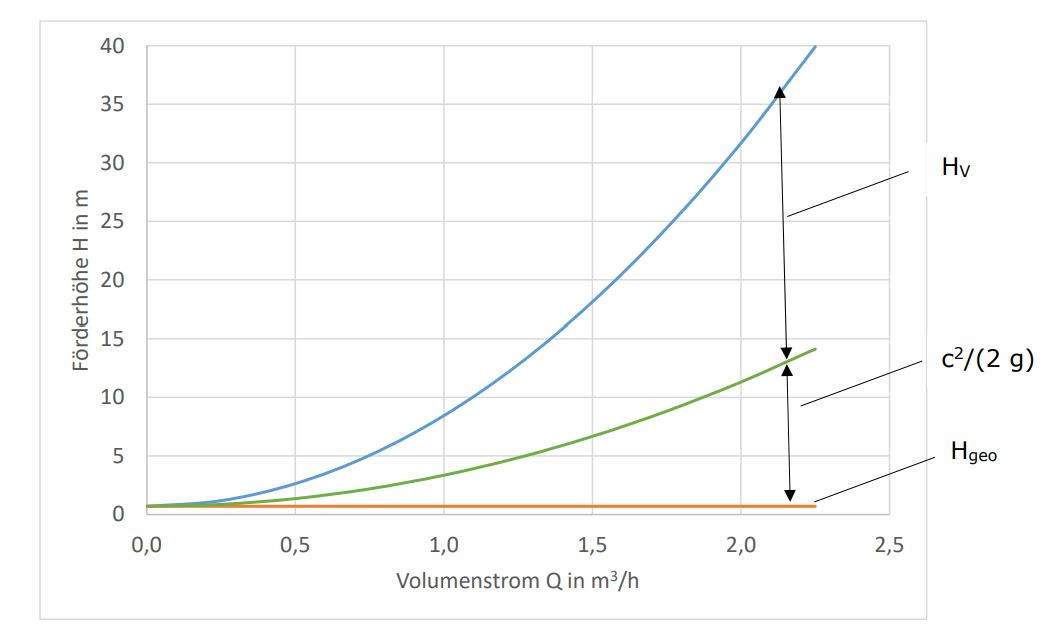
\includegraphics[width=0.7\textwidth]{Abbildungen/Rohrleitungskennlinie}
		\caption{Rohrleitungskennlinie bei vollständig geöffneter Düse}
		\label{fig:230512_Rohrleitungskennlinie}
\end{figure}
%
\subsection{Proportionalität zwischen Leistung und Drehzahl}
\label{subsec:P_mech-n}
Die mechanische Leistung $P_{Mech.}$ ist in \autoref{eq:230512_MechanischeLeistung} definiert.
%
\begin{equation}
	P_{Mech.}= M \cdot 2 \cdot \pi \cdot n
\label{eq:230512_MechanischeLeistung}
\end{equation}
%
Dabei ist $n$ die Drehzahl und $M$ das Moment, somit ist die mechanische Leistung proportional zu der Drehzahl.
\subsection{Einstellungsmöglichkeiten für den Betriebspunkt}
Der Betriebspunkt ist mit dem Volumenstrom/Strahldurchmesser, durch eine angelegte Last am Generator oder den Erregerstrom $I_{Err}$ steuerbar. Dabei ist der optimale Betriebspunkt über die optimale Drehzahl zu ermitteln. Die optimale Drehzahl liegt bei der halben Austrittsgeschwindigkeit der Düse.

\subsection{Regelung über hydraulischen Parameter}
Die Düsennadel kann so eingestellt werden, dass sich der Durchflussquerschnitt verändert. Mit dem Durchflussquerschnitt lässt sich dann der Volumenstrom Q steuern und somit die Drehzahl der Pelton-Turbine.